\documentclass[a4paper,12pt]{article}
\usepackage[utf8]{inputenc}
\usepackage[czech]{babel}
\usepackage[T1]{fontenc}
\usepackage{graphicx}
\usepackage{array}
\usepackage{booktabs}
\usepackage{tabularx}
\usepackage{makecell}
\usepackage{float}
\usepackage{url}
\usepackage{listings}
\usepackage{xcolor}
\usepackage{diagbox}
\usepackage{hyperref}
\newcommand{\centered}[1]{\begin{tabular}{l} #1 \end{tabular}}
\newcommand{\unit}[1]{\ensuremath{\, \mathrm{#1}}}
\addto\captionsczech{\renewcommand{\refname}{Seznam použité literatury}}
\addto\captionsczech{\renewcommand{\figurename}{\textbf{Obrázek}}}
\addto\captionsczech{\renewcommand{\tablename}{\textbf{Tabulka}}}
\renewcommand{\lstlistingname}{\textbf{Kód}}

\lstset{
    language=Python,
    basicstyle=\ttfamily\footnotesize,  % Zmenšené písmo
    keywordstyle=\color{blue},
    commentstyle=\color{gray},
    stringstyle=\color{red},
    numbers=left,
    numberstyle=\tiny\color{gray},
    stepnumber=1,
    breaklines=true,
    frame=single
}

\begin{document}
\vspace{\fill}
\begin{center}
    \renewcommand{\arraystretch}{1.75}
    \begin{tabularx}{\textwidth}{|X|X|X|}
        \hline
        \multicolumn{1}{|c|}{\rule{0pt}{2.25cm} 
\includegraphics[height=2cm]{img/ctu_logo.png}} & 
        \multicolumn{2}{c|}{\makecell{\textbf{KATEDRA FYZIKY}}} \\
        \hline
        \multicolumn{3}{|c|}{\Large \textbf{\centered{LABORATORNÍ CVIČENÍ Z FYZIKY}}} \\
        \hline
        \multicolumn{2}{|X}{\small{Jméno} \newline \textbf{Pavel Pernička}} & \multicolumn{1}{|X|}{\small{Datum měření} \newline \textbf{17.4.2025}} \\
        \hline
        {\small{Semestr} \newline \textbf{Letní 2025}} & {\small{Ročník} \newline \textbf{1.}} & {\small{Datum odevzdání} \newline \textbf{6.5.2025}} \\
        \hline
        {\small{Stud. skupina} \newline \textbf{6}} & {\small{Lab. skupina} \newline \textbf{1031}} & {\small{Klasifikace} \newline}\\
        \hline
        \multicolumn{3}{|c|}{\rule{0pt}{1cm}} \\
        \hline
        \multicolumn{1}{|X|}{\small{Číslo úlohy \newline \textbf{8}}} &
        \multicolumn{2}{|p{8cm}|}{\small{Název úlohy \newline \textbf{Studium mechanických kmitů -- Pohlovo
kyvadlo}}} \\

        \hline
    \end{tabularx}
\end{center}

\newpage

\section{Úkol měření}
\begin{enumerate}
    \item Proměřte kmitočtové charakteristiky nucených kmitů Pohlova kyvadla pro různá tlumení.
    \item Změřte koeficient útlumu a periodu volných kmitů Pohlova kyvadla pro různá tlumení.
\end{enumerate}

\section{Seznam použitých přístrojů}
\begin{itemize}
    \item Stopky
    \item Pohlovo kyvadlo
\end{itemize}
\section{Měření}
\subsection{Postup}
\begin{enumerate}
    \item Zapneme elektromotor připojený k aparatuře kyvadla
    \item Pomocí měření času 10 otáček při různých napětích na motoru zjistíme závislost budící frekvence na napětí.
    \item Pro několik různých budících frekvencí měříme amplitudu ručičky kyvadla. Měříme výchylky na obou stranách, z nich vytvoříme průměr. Volíme různá nastavení tlumení:
        \begin{itemize}
            \item Brzdící elektromagnet je zcela odpojen ($I_{B0} = 0$)
            \item Proud tekoucí elektromagnetem je $I_{B1}=0,25A$
            \item Proud tekoucí elektromagnetem je $I_{B2}=0,40A$
            \item Proud tekoucí elektromagnetem je $I_{B3}=0,55A$
            \item Proud tekoucí elektromagnetem je $I_{B4}=0,90A$
        \end{itemize}
    \item Vypneme elektromotor
    \item Pro stejné nastavení brzdícího elektromagnetu jako výše opakovaně změříme čas 10 kmitů při manuálním natažení ručičky kyvadla do krajní pozice stupnice.
    \item Během měření předchozího bodu si zapisujeme posloupnost výchylek na jedné ze stran stupnice.
\end{enumerate}

\subsection{Naměřené hodnoty}

\begin{table}[H]
    \centering
    \renewcommand{\arraystretch}{1.5}
    \begin{tabular}{|c|c|c|}
        \hline
        \textbf{\#} & \textbf{$U$ [V]} & \textbf{Čas 10 otáček $t_{10}$ [s]} \\ \hline
        1 & 4,6 & 29,74 \\ \hline
        2 & 10,5 & 11,95 \\ \hline
        3 & 15,0 & 7,91 \\ \hline
        4 & 12,1 & 10,11 \\ \hline
    \end{tabular}
    \caption{Závislost otáček na napětí}
    \label{tab:frekvence}
\end{table}

\begin{table}[H]
    \centering
    \renewcommand{\arraystretch}{1.5}
    \begin{tabular}{|c|c||c|c||c|c||c|c||c|c||c|c|}
        \hline
        \textbf{\#} & \textbf{$U$ [V]} 
        & \multicolumn{2}{c||}{$A(I_{B0})$} 
        & \multicolumn{2}{c||}{$A(I_{B1})$} 
        & \multicolumn{2}{c||}{$A(I_{B2})$} 
        & \multicolumn{2}{c||}{$A(I_{B3})$} 
        & \multicolumn{2}{c|}{$A(I_{B4})$} \\
        & & $A+$ & $A-$ & $A+$ & $A-$ & $A+$ & $A-$ & $A+$ & $A-$ & $A+$ & $A-$ \\ \hline
        1 & 4,0 & -0,1 & 1,2 & -0,1 & 1,2 & -0,1 & 1,3 & -0,1 & 1,2 & -0,1 &  1,2 \\ \hline
        2 & 6,3 & -1 & 2 & -1 & 2,1 & -1 & 2,2 & -0,9 & 2,1 & -1 & 2 \\ \hline
        3 & 6,9 & -2 & 3 & -2,2 & 3,1 & -9 & 10 & -2 & 3 & -1,2 & 2,2 \\ \hline
        4 & 7,5 & -6 & 7,2 & -7,3 & 8,9 & -7 & 8 & -4,1 & 5,3 & -2 & 3 \\ \hline
        5 & 8,0 & -20 & 20 & -16 & 17 & -8 & 9 & -5 & 6,1 & -2 & 3 \\ \hline
        6 & 9,0 & -20* & 20* & -2 & 3 & -1 & 2,1 & -1 & 2,2 & -1 & 2 \\ \hline
        7 & 9,7 & -7 & 8 & -0,3 & 1,9 & -0,2 & 1,9 & -0,2 & 1,3 & -0,1 & 1,3 \\ \hline
        8 & 11,0 & -0,1 & 1,2 & 0 & 1,1 & 0 & 1,1 & 0 & 1,1 & 0 & 1,1 \\ \hline
    \end{tabular}
    \caption{Závislost amplitudy na napětí na elektromotoru při různých brzdných proudech}
    \label{tab:amplituda}
\end{table}

\begin{table}[H]
    \centering
    \renewcommand{\arraystretch}{1.5}
    \begin{tabular}{|c|c|c|c|}
        \hline
        \textbf{\#} & \textbf{$T_{10}(I_{B0})$ [s]} & \textbf{$T_{10}(I_{B1})$ [s]} & \textbf{$T_{10}(I_{B2})$ [s]} \\ \hline
        1 & 17,18 & 17,27 & 17,25 \\ \hline
        2 & 17,50 & 17,14 & 17,30 \\ \hline
        3 & 17,49 & 17,22 & 17,13 \\ \hline
    \end{tabular}
    \caption{Perioda kmitů kyvadla při počáteční pozici v maximu stupnice a různých brzdných proudech, $t=10\ s$}
    \label{tab:perioda}
\end{table}

\begin{table}[H]
    \centering
    \renewcommand{\arraystretch}{1.5}
    \begin{tabular}{|c|c|c||c|c|c||c|c|c||c|c|c||c|c|c|}
        \hline
        \multicolumn{3}{|c||}{$A(I_{B0})$} 
        & \multicolumn{3}{c||}{$A(I_{B1})$} 
        & \multicolumn{3}{c||}{$A(I_{B2})$} 
        & \multicolumn{3}{c||}{$A(I_{B3})$} 
        & \multicolumn{3}{c|}{$A(I_{B4})$} \\ \hline
        \textbf{1} & \textbf{2} & \textbf{3} 
        & \textbf{1} & \textbf{2} & \textbf{3} 
        & \textbf{1} & \textbf{2} & \textbf{3} 
        & \textbf{1} & \textbf{2} & \textbf{3} 
        & \textbf{1} & \textbf{2} & \textbf{3} \\ \hline
        19 & 18 & 19 & 18 & 18 & 18 & 18 & 17 & 17 & 15 & 15 & 15 & 11 & 11 & 11 \\ \hline
        18 & 18 & 18 & 17 & 17 & 14 & 18 & 17 & 17 & 12 & 12 & 12 & 6 & 7 & 6 \\ \hline
        17 & 17 & 17 & 16 & 16 & 15 & 13 & 13 & 13 & 9 & 9 & 9 & 4 & 4 & 4 \\ \hline
        16 & 16 & 16 & 15 & 15 & 14 & 11 & 11 & 11 & 7 & 7 & 8 & 3 & 3 & 3 \\ \hline
        16 & 15 & 16 & 14 & 14 & 14 & 9 & 9 & 9 & 5 & 6 & 5 & 2 & 2 & 2 \\ \hline
        14 & 14 & 15 & 13 & 13 & 13 & 8 & 8 & 8 & 4 & 4 & 4 & 1 & 1 & 1 \\ \hline
        14 & 13 & 14 & 12 & 12 & 12 & 7 & 7 & 6 & 3 & 3 & 2 & 1 & 1 & 1 \\ \hline
        13 & 13 & 13 & 11 & 10 & 11 & 6 & 5 & 6 & 2 & 2 & 3 & 1 & 1 & 1 \\ \hline
    \end{tabular}
    \caption{Posloupnost amplitudových výchylek v čase ve zvolených brzdných proudech}
    \label{tab:posloupnost}
\end{table}

\section{Výpočty}

Pro výpočet logaritmického dekrementu $\Lambda$ a koeficientu $\delta$ použijeme vzorce odvozené ze zadání:

\begin{itemize}
    \item Logaritmický dekrement: $$ \Lambda = \ln\left( \frac{x(t)}{x(t+T)} \right) $$
    \item Koeficient \(\delta\): $$ \delta = \frac{\Lambda}{T} $$
\end{itemize}

Na základě měření v tabulce \ref{tab:posloupnost}, kde jsme zprůměrovali amplitudu v obou stranách, a vzorců výše byly pro jednotlivé hodnoty brzdného proudu $I_B$ stanoveny veličiny v tabulce \ref{tab:shrnutihodnoty}

\begin{table}[H]
    \centering
    \renewcommand{\arraystretch}{1.5}
    \begin{tabular}{|c|c|c|c|c|}
        \hline
        \textbf{$I_B$ [A]} & \textbf{$T$ [s]} & \textbf{$f$ [Hz]} & \textbf{$\Lambda$} & \textbf{$\delta$} \\ \hline
        0.00 & 1.739 & 0.575 & 0.0541 & 0.0311 \\ \hline
        0.25 & 1.721 & 0.581 & 0.0000 & 0.0000 \\ \hline
        0.40 & 1.723 & 0.580 & 0.0572 & 0.0332 \\ \hline
        0.55 & 1.700 & 0.588 & 0.0000 & 0.0000 \\ \hline
        0.90 & 1.680 & 0.595 & 0.0000 & 0.0000 \\ \hline
    \end{tabular}
    \caption{Přehled vypočtených hodnot $T$, $f$, $\Lambda$ a $\delta$ pro jednotlivé hodnoty brzdného proudu $I_B$}
    \label{tab:shrnutihodnoty}
\end{table}

\section{Grafy}
\begin{figure}[H]
    \centering
    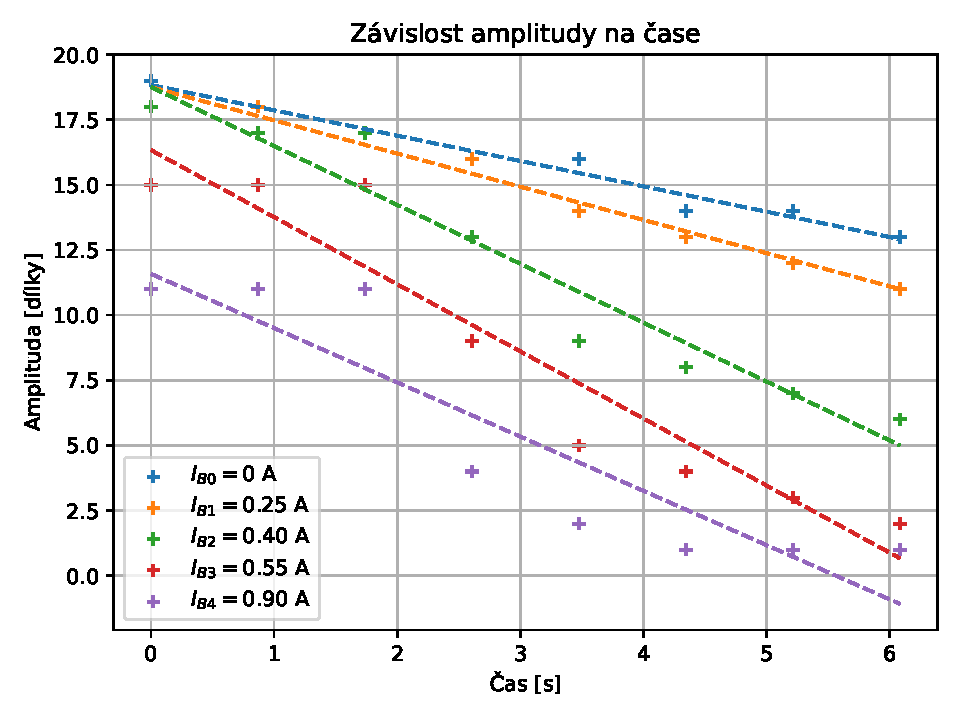
\includegraphics[width=0.9\textwidth]{img/amp_cas.pdf}
    \caption{Závislost amplitudy kyvadla na čase pro různá tlumení $I_B$. Body odpovídají naměřeným hodnotám, přímky byly získány metodou nejmenších čtverců.}
    \label{fig:ampl_cas}
\end{figure}

\begin{figure}[H]
    \centering
    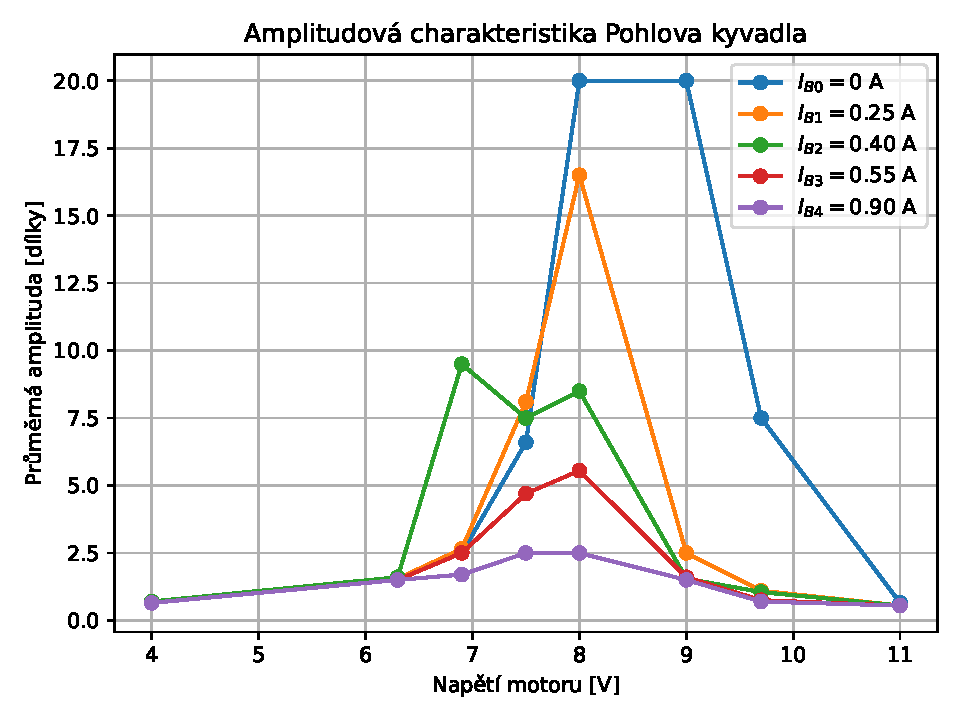
\includegraphics[width=0.9\textwidth]{img/amp_char.pdf}
    \caption{Amplitudová charakteristika Pohlova kyvadla pro různá tlumení $I_B$.}
    \label{fig:amp_char}
\end{figure}

\section{Závěr}
Cílem úlohy bylo experimentálně ověřit chování Pohlova kyvadla při volném i~nuceném kmitání a~stanovit kmitočtové charakteristiky a útlumové konstanty pro různá nastavení tlumení.
Pomocí grafů naměřených hodnot jsme ověřili, že s rostoucím brzdným proudem $I_B$ dochází ke snižování maximálních amplitud a ke zvyšování míry tlumení. Z amplitudových charakteristik byla patrná rezonance u nižších hodnot tlumení, s~rostoucím tlumením se rezonanční amplituda výrazně snižovala a křivka zplošťovala. 

U malého tlumení bylo možné určit logaritmický dekrement $\Lambda$ a koeficient útlumu $\delta$ s dostatečnou přesností. U většího tlumení byl pokles amplitudy mezi maximy příliš malý a~výpočet $\Lambda$ nebyl možný bez větší nejistoty. Tyto nejistoty je obtížné objektivně odhadnout, protože samotné Pohlovo kyvadlo se chovalo poměrně nepředvídatelně a reakční doba lidského faktoru při odečítání výchylek byla neuspokojivá. 

\begin{thebibliography}{}

    \bibitem{pohl}
    Milan Červenka. \textit{Studium mechanických kmitů -- Pohlovo
kyvadlo}. Laboratorní úloha, 2013. Dostupné online: \url{https://planck.fel.cvut.cz/praktikum/downloads/navody/pohl.pdf}.

    \bibitem{zpracdat}
    Milan Červenka. \textit{Zpracování fyzikálních měření}. Studijní text pro fyzikální praktikum, 2020. Dostupné online: \url{https://planck.fel.cvut.cz/praktikum/downloads/navody/zpracdat.pdf}.

\end{thebibliography}

\end{document}
